% !TeX spellcheck = en_GB
\def\ChapterTitle{}

\chapter{Multi-Domain Trust Assessment in Collaborative Marine \glspl{manet}}
\label{ch:multi_domain}
\lhead{Chapter \thechapter. \emph{\nameref{ch:multi_domain}}}

\section{Introduction}

Having validated the premises a fair analogue can be generated between RF and \gls{uan} \glspl{manet} (\autoref{q:rfuan}), that those networks can have communications trust management applied to them with the aid of machine learning (\autoref{q:uantmf}, \autoref{q:ml}), and that there are strong indications that physical mobility can be applied as an additional trust management domain (\autoref{q:phys}), now the ability to meaningfully join these domains will be demonstrated (\autoref{q:joint}) and their performance assessed (\autoref{q:perf}).

A key question in this chapter is to assess the advantages and disadvantages of utilising trust from across domains for \gls{mtfm}. 
This includes a secondary question as to how trust assessments from these domains are most effectively combined or synthesised. 

This work is separated into three main experiments;
\begin{itemize}
	\item \autoref{sec:mdt_defined} - Optimisation of a simple concatenation of trust domain metric vectors with respect to each misbehaviour (using the same methodology as \autoref{ch:comms_trust})
	\item \autoref{sec:mdt_alternate} - Classification Performance Assessment of these domains (as well as proposed ``Alternate'' metric groupings)
	\item \autoref{sec:mdt_synthetic} - Classification Performance Assessment of a Generalised Synthetic Domain approach to per-misbehaviour training
\end{itemize}

\section{Initial Optimisation of Multi-Domain Trust with Predefined Domains}\label{sec:mdt_defined}

In this first experiment, the trust domains established previously in \autoref{ch:comms_trust} and \autoref{ch:physical_trust} are combined as a single metric weighting vector for \gls{mtfm} operation.

The communications domain metric vector is constructed using those trust metrics that are applicable to the marine environment from~\cite{Guo2012}, as the simulated marine acoustic modem stack does not operate on the same tiered data-rate approach as used in the 802.11 stack, the data rate metric was not included. Remaining metrics are; Delay, Received and Transmitted power, Throughput ($S$), Offered Load ($G$) and \gls{plr}.

Thus, the metric vector used for communications-trust assessment is;

\begin{equation}
  X_{comms}=\{D, P_{RX}, P_{TX}, S, G, PLR\}
  \label{eq:comms_vector}
\end{equation}

From \autoref{ch:physical_trust}; Three physical metrics are selected to encompass the relative distributions and activities of nodes within the network; \gls{indd}, \gls{inhd}, and Node Speed. These metrics encapsulate the relative distributions of position and velocity within the fleet, optimising for the detection of outlying or deviant behaviour within the fleet.

Conceptually, \gls{indd} is a measure of the average spacing of an observed node with respect to its neighbours. \gls{inhd} is a similar approach with respect to node orientation.

\begin{align}
  INDD_{i,j} &= \frac{|P_j - \sum_x \frac{P_x}{N}|}{\frac{1}{N}\sum_x \sum_y{|P_x - P_y| (\forall x \neq y)}}\\
  INHD_{i,j} &= \hat{v} \vert v= V_j - \sum_x{\frac{V_x}{N}}\\
  V_{i,j} &= |V_j|
\end{align}

Thus, the metric vector used for physical-trust assessment is;

\begin{equation}
  X_{phy}=\{\text{INDD}, \text{INHD}, V\}
  \label{eq:phys:vector}
\end{equation}

This simplest possible combination is a vector concatenation across domain metric vectors; in this case; 

\begin{equation}
  X_{full} =  (X_{comms}|X_{phy}) = \{D, P_{RX}, P_{TX}, S, G, PLR, \text{INDD}, \text{INHD}, V\}
  \label{eq:merge:vector}
\end{equation}


\subsection{Metric Weight Analysis Scheme}

From \autoref{eq:metric_weighting}, the final trust values arrived at using \gls{mtfm} are dependent on metric values, the weights assigned to each metric, and the structure of the $g$, $b$ comparison vectors.

This permits the assessment of the significance of different metrics in the detection and identification of different behaviours. 
The primary aspects of a (mis)behaviour can be detected and assessed by comparing a weighted trust assessment against the deviation from a control result set (``fair'' node behaviour) using the same weight, i.e.\ we are interested in the weight schemes that create the largest difference between fair and misbehaving cases.

For a metric weight vector $H$, where the metric $m_j$ is emphasised as being twice as important as the other metrics, an initial weighting vector $H'=[h_i\cdots h_M]$ is formed such that $h_i = 1 \forall i \ne j; h_j=2$. 
That vector $H'$ is then scaled such that $\sum H = 1$ by $H= \frac{H'}{\sum |H'|}$.

The construction of the $g$ and $b$ vectors from~\autoref{eq:grc} depends on the particular metric, e.g. Throughput ($S$) on a link is assumed to be positively correlated to trustworthiness and so follows the default construction ($g(S) \mapsto \max, b(S) \mapsto \min$), whereas in the case of a metric such as delay, this relationship is inverted, i.e.\ longer delays indicate less trustworthy activity ($g(D) \mapsto \min, b(D) \mapsto \max$).
This inversion relationship (i.e.\ those with the construction $g(x) \mapsto \min, b(x) \mapsto \max$) is signified by a negative weights in the $H$ vector.

This signed $H$ vector reflects the search space of this analysis; probing the multi-dimensional metric search space for metric combinations the create the largest deviations in Trust assessment under node misbehaviour.

In complex environments, the relationship between metrics trustworthiness correlations is not always as obvious as the throughput / delay examples.
This phenomenon was mentioned by~\citet{Guo2012}, but was manually configured for each metric for each behaviour and no analytical method for quantitatively establishing such relationships has been presented since.

With the nine selected metrics from across communications and physical behaviours, we can explore this metric space by varying the weights associated with each metric, and choose to emphasise across three levels; i.e.\ metrics can be ignored or over-emphasised. Naively this results in $3^9 = 19683$ combinations, however as these weights are being normalised, redundant duplicates can be eliminated, e.g. $[0,0,0,0,1,0,0,0,0] \equiv [0,0,0,0,2,0,0,0,0]$ leaving 18661 unique weights for analysis.

To assess the performance of a given weight combination (i.e.\ an optimisation factor), we are initially interested in the metric weight vector that consistently provides the largest deviation in the final trust value $T$ across the cohort, i.e.\ producing the most clear detection of a node misbehaving in that particular fashion.
This is approached as an inverse outlier filtering problem, and the range outside a $\pm\sigma$ envelope compared to the equivalent weighting in a known ``fair'' behaviour is selected to assess detection (or comparing to other misbehaviours to assess discrimination).
See~\autoref{sec:metric_weighting}.
Note that at this point we establish ``signatures'' of different behaviours rather than optimal detection weights.

We apply a Random Forest regression~\cite{Breiman2001} to assess the relative importance of the selected metrics on relative detectability of malicious behaviour. 
Random Forest accomplishes this by generating a large number of random regression trees and prune these trees based on how accurate they are in correctly matching the input data.
In this case that data is the deviation in trust observed ($\Delta T$) between a two behaviours, i.e. maximising the ability to tell the difference between two given behaviours (i.e.\ ``Fair'' and ``Malicious'').
A major advantage of Random Forest in this case is that by walking the most successful regression trees, we can acquire an already normalised maximal activation weight for the particular behaviour comparison being tested.

After establishing the importance of weights in particular behaviours, a final weight is arrived at by algorithmically those few metrics that are important, rather than having to further explore the computationally expensive weight-space.

Using this approach, the results of these simulations can be explored, condensing the multi-dimensional problem (target / observer / behaviour / metric / time) down to a more manageable level for analysis.

\subsection{Results and Discussion}

Figs~\ref{fig:comms_feature_extraction} and~\ref{fig:phys_feature_extraction}, show the resultant feature significances for Communications -only and Physical only metric selections respectively, and in ~\autoref{fig:multi_feature_extraction}, these metric spaces are brought together and reassessed.
Firstly, when the domains are brought together, the communications domain appears to largely dominate significance, with SlowCoach being the only behaviour where the significance of a Physical metric comes close to the assessed significance of communications metrics.
While this does not initially bode well for the overall utility of the physical metrics use in tandem with the communications domain, it may be that these physical metrics become key deciding factors between conceptually similar behaviours; in \autoref{fig:multi_feature_extraction}, both the Shadow and SlowCoach behaviours have a highly significant transmission power factor, but SlowCoach also exhibits a significant Speed factor where Shadow does not.

In the next experiment, weighting filters based both these initial domains and a proposed pair of ``Alternate'' domains are assessed for their blind operation and performance.


% These figures are the output of test_Thesis_Diagrams.test????Relevance
\begin{figure}[h!]
  \centering
  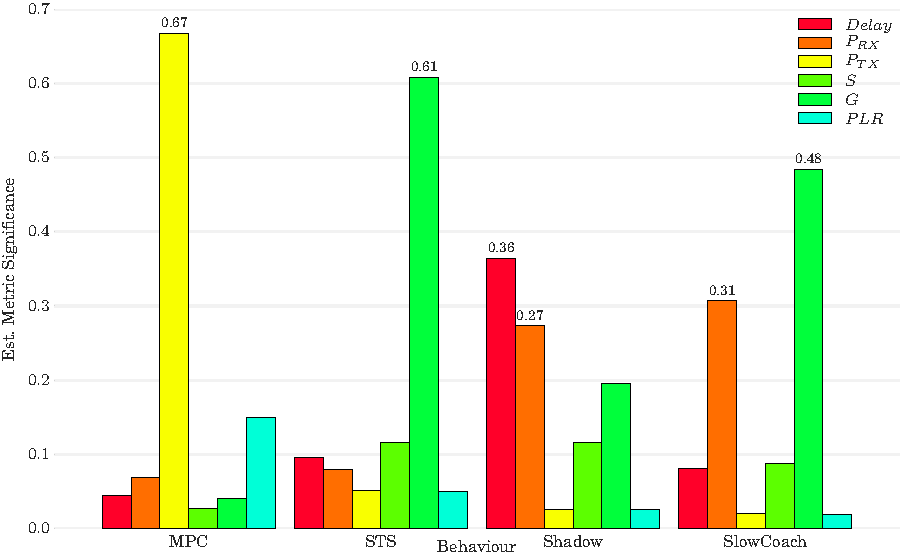
\includegraphics[width=\linewidth]{comms_metric_trust_relevance}
  \caption{Communications Metric Features ($X_{comms}$)}
  \label{fig:comms_feature_extraction}
\end{figure}

\begin{figure}[h!]
  \centering
  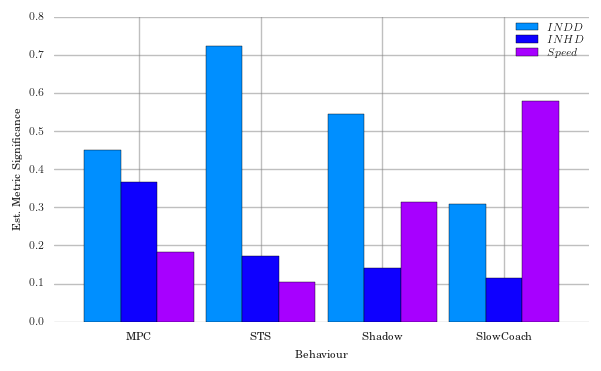
\includegraphics[width=\linewidth]{phys_metric_trust_relevance}
  \caption{Physical Metric Features ($X_{phys}$)}
  \label{fig:phys_feature_extraction}
\end{figure}

\begin{figure}[h!]
  \centering
  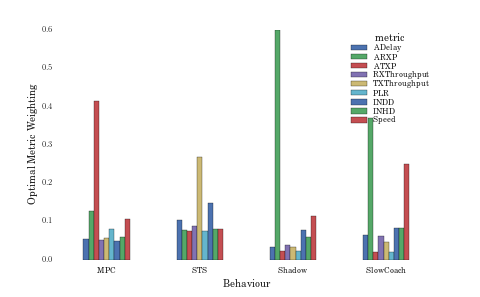
\includegraphics[width=\linewidth]{full_metric_trust_relevance}
  \caption{Multi Domain  Metric Features ($X_{merge}$)}
  \label{fig:multi_feature_extraction}
\end{figure}

\begin{table}
  \centering
  \caption{Multi Domain Metric Feature Correlation ($X_{merge}$)}
  \begin{tabular}{lrrrrrrrrr}
\toprule
{} &  $Delay$ &  $P_{RX}$ &  $P_{TX}$ &  $T^P_{RX}$ &  $PLR$ &  $T^P_{TX}$ &  $INDD$ &  $INHD$ &  $Speed$ \\
Misbehaviour &          &           &           &             &        &             &         &         &          \\
\midrule
MPC          &   -0.187 &     0.129 &     0.579 &       0.006 &  0.069 &      -0.146 &   0.040 &  -0.190 &   -0.297 \\
STS          &   -0.195 &    -0.035 &     0.019 &      -0.100 &  0.019 &       0.381 &  -0.209 &   0.057 &    0.062 \\
Shadow       &    0.004 &    -0.654 &     0.030 &      -0.016 &  0.030 &       0.063 &   0.120 &   0.158 &    0.266 \\
SlowCoach    &   -0.157 &    -0.533 &     0.013 &      -0.132 &  0.013 &      -0.028 &   0.159 &   0.206 &    0.460 \\
\bottomrule
\end{tabular}

  \label{tab:full_metric_correlations}
\end{table}



\section{Performance Assessment and Alternative Domain Groupings}\label{sec:weight_assessment}\label{sec:mdt_alternate}

In both single-domain cases in the previous section, there are clear ``signatures'' in misbehaviours that don't directly target that domain ($P_{RX}$ in the Physical Shadow and Slowcoach behaviours in Fig~\ref{fig:comms_feature_extraction} and $INDD$ in the Selfish Target Selection behaviour in Fig~\ref{fig:phys_feature_extraction}).
This inter-domain activity is to be expected in \glspl{manet} in general, where the physical reality of the network (i.e.\ distance between nodes) directly impacts the behaviour of the logical communications network (i.e.\ delay between nodes), and is a useful characteristic coupling for differentiating potential misbehaviours.

\autoref{fig:alternate_domain_diag} attempts to lay out the results of Feature Extraction across a spectrum of Communications / Physical domain assessment, matching the assumed domains of the stated misbehaviours based on the resultant significance in relevant domain misbehaviours.
From this, two alternative ``domains'' are constructed; ``Comms. Alt.'' and ``Phys. Alt.'', as artificial constructions of the relevant domains attempting to encapsulate the most responsive features for each misbehaviour-domain\footnote{These constructions are largely arbitrary and are the result of ``extensive'' analysis by the author and their supervisors application of the MK I Eyeball}.

This gives 5 candidate metric ``domains'' for optimisation and performance assessment;

\begin{align}
	X_{full} &=  (X_{comms}|X_{phy}) = \{D, P_{RX}, P_{TX}, S, G, PLR, \text{INDD}, \text{INHD}, V\}\\
    X_{comms} &=\{D, P_{RX}, P_{TX}, S, G, PLR\}\\
    X_{phy} &=\{\text{INDD}, \text{INHD}, V\}\\
	X_{comms}^` &= \{P_{TX}, S, G, PLR, \text{INDD}\} \label{eq:comms_alt_vector}\\
	X_{phys}^` &= \{D, P_{RX}, \text{INDD}, \text{INHD}, V\} \label{eq:phys_alt_vector}
\end{align}

\begin{figure}[h]
	\centering
	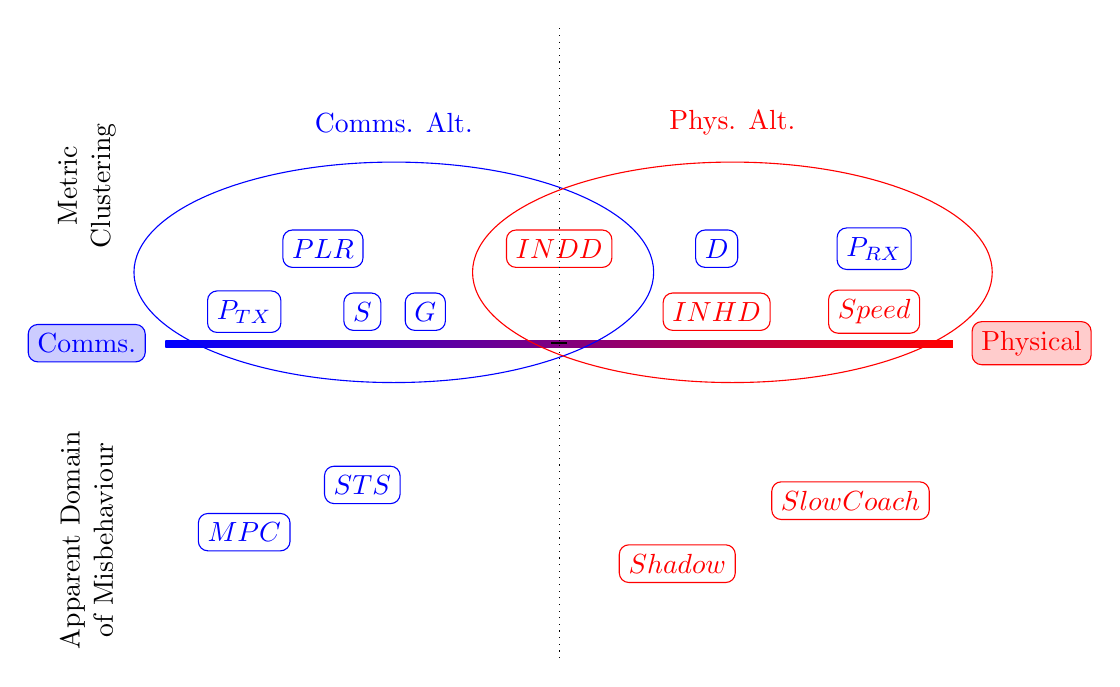
\begin{tikzpicture}[-latex,
	comms/.style={text=blue, draw=blue, rounded corners=.8ex},
	phys/.style={text=red, draw=red, rounded corners=.8ex}]
	% Start off with the line
	%\draw [<-|][comms, draw=blue, very thick] (0,1) -- (5,1); 
	%\draw [|->][phys, draw=red, very thick] (5,1) -- (10,1); 
	\path[left color=blue,right color=red]
	(0,0.95) rectangle +(10,2.5pt);
	
	% Baseline labels
	\node[comms, fill=blue, fill opacity=0.2, text opacity=1] at (-1,1) {Comms.};
	\node[phys, fill=red, fill opacity=0.2, text opacity=1] at (11,1) {Physical};
	
	% Metric Labels
	\node[comms] at (7,2.2) {$D$};
	\node[comms] at (9,2.2) {$P_{RX}$};
	\node[comms] at (1,1.4) {$P_{TX}$};
	\node[comms] at (2.5,1.4) {$S$};
	\node[comms] at (3.3,1.4) {$G$};
	\node[comms] at (2,2.2) {$PLR$};
	\node[phys] at (5,2.2) {$INDD$};
	\node[phys] at (7,1.4) {$INHD$};
	\node[phys] at (9,1.4) {$Speed$};
	
	\node[rotate=90, align=center] at (-1, 3) {Metric\\Clustering};
	\node[rotate=90, align=center] at (-1, -1.5) {Apparent Domain\\of Misbehaviour};
	\node[comms] at (1,-1.4) {$MPC$};
	\node[comms] at (2.5,-0.8) {$STS$};
	\node[phys] at (6.5,-1.8) {$Shadow$};
	\node[phys] at (8.7,-1) {$SlowCoach$};
	
	% Draw approx subsets
	\draw[comms] (2.9,1.9) ellipse (3.3 and 1.4);
	\draw[phys] (7.2,1.9) ellipse (3.3 and 1.4);
	
	\node[text=red] at (7.2,3.8) {Phys. Alt.};
	\node[text=blue] at (2.9,3.8) {Comms. Alt.};
	
	% Misc
	\draw[-|][dotted] (5,5) -- (5,1);
	\draw[-|][dotted] (5,-3) -- (5,1);
	
	
	\end{tikzpicture}
	\caption{Assumptions made about the relevant domains of impact / detectability of misbehaviours, and domain relevance of metrics, may not be optimal}
	\label{fig:alternate_domain_diag}
\end{figure}

From the significance information resulting from the previous section, an ``estimated'' signature for each behaviour can be inferred, which can then be fed back into \gls{mtfm}. 
The aim of this iteration is to minimise the number of weight permutations required to come to a conclusion about the behaviour under observation. 

However, these approximated signatures have no information regarding the ``sign'' of the  $g$,$b$ comparison vectors from \autoref{eq:metric_weighting}, i.e.\ there is no hint as to whether the relationship is $g(x) \mapsto \max, b(x) \mapsto \min$ or $g(x) \mapsto \min, b(x) \mapsto \max$)  

One option would be to go back to the regression point and expand the combination options to include negative values, signifying inverted $g,b$ relationships, however this is combinatorially explosive.\footnote{The current version of this analysis uses three metric weights; ignored, standard, emphasised, giving $3^9 = 19683$ combinations. Expanding this to include inverted standard and inverted emphasised weights would raise that to $5^9 = 1.9\times 10^6$ for each training dataset for each node relationship}
Instead, the ``significance'' weight is permuted against it's possible combinations of ``flips'', i.e.\ for $X_s=[0.3,0.4,0.01,0.02,0.27]$ could also be $X_s^p=[0.3,-0.4,0.01,0.02,0.27]$ and so on. 
This sign permutation is filtered based on a threshold value ($0.01$), so for all indices below that threshold will not be permuted on, halving the number of combinations required for each indices eliminated.
This reduces the number of additional assessments required from $1.9\times 10^6$ to approximately 500 (when applied to all nine metrics) for each experimental run.

The best of these permutations is selected to both maximise the (correct) deviation between each nodes trust perspectives and to minimise the trust value reported for the misbehaving nodes; $\Delta T \to \max^+$ (\autoref{eq:delta_t}, results summarised in \autoref{tab:domain_deltas}).
Additionally, a ``False Positive'' assessment, $\Delta T^-$ (\autoref{eq:delta_t_minus} shown in \autoref{tab:domain_deltas_minus}) which encapsulates the average false positive selection rate.

\begin{align}
  \Delta T_{ix} &= \frac{\sum_{j\neq x}\left( \overline{T_{i,j}}^{\forall t}\right)}{N-1} - \overline{T_{i,x}}^{\forall t} \label{eq:delta_t}\\
  \Delta T_{ix}^- &= \frac{\sum_{j\neq x} \Delta T_{ij}}{N-1} - \overline{\Delta T_{i,x}}^{\forall t} \label{eq:delta_t_minus} 
\end{align}

Where $i$ is a given observer, $x$ is the known misbehaving node, $\overline{T_{i,j}}^{\forall t}$ is the average weighted trust assessment of node $j$ observed by node $i$ across time and $N$ is the number of nodes.

Conceptually, $\Delta T_{ix}$ represents the ``Relative Distrust'' of the target node $x$, as the difference in trust value from $0\to1$, the higher the value the larger the ``drop'' in trst of the misbehaviour compared to the cohort. 
$\Delta T_{ix}^-$ represents the average $\Delta T_{ij}$ for all other nodes, representing the likelihood of another node being as highly distrusted as $x$, where positive values indicate that $x$ is not the obvious outlier, negative values indicate that $x$ is a very clear outlier, and near-zero values indicate a difficulty in selection of any outlier from the cohort.

The ``best'' weight permutations, as shown in \autoref{tab:optimised_weights}, are applied to untrained datasets for these results.

This is a departure from the Dixons Q-Test applied in \autoref{ch:physical_trust}, as the number of metrics in use, and the recognised variability in response to different metrics makes a simple outlier assessment unfairly naive for performance assessment. 
With respect to \ref{q:ml} and \ref{q:joint}, the primary motivation to this work is to generate weights that (in the case of a single attacker) induce the largest Trust reduction observable by as many nodes within the network.
This motivation is encapsulated in the $\Delta T_{ix}$ assessment, and allows increased abstraction so as to assess the variability of metrics in use, and to assess the usefulness of such generated ``Alternate'' or ``Synthetic'' domains.

An exemplar subset of the results is shows in Figs~\ref{fig:comms_time_mpc}-~\ref{fig:full_time_slowcoach}, with the ``misbehaving node'' indicated above its distribution plot.

The most intuitively ``Communications'' behaviour, \gls{mpc}, scores comfortably in the 90th percentile range in both Communications Domain (\autoref{fig:comms_time_mpc}) and Full Domain (\autoref{fig:full_time_mpc})  trust assessments. As seen in \autoref{tab:optimised_weights}, both the ``Full'' and ``Comms'' metric optimisations heavily weigh $P_{TX}$, and as this is the metric directly modified by the misbehaviour, it is expected that this is easily discernible using these domain weights.
However when this communications information is unavailable, as is the case in the use of Physical Domain metrics alone in \autoref{fig:phys_time_mpc}, the misbehaving node (Alfa) is completely indiscernible compared to the other nodes, with all nodes in the cohort tending to a trust value of $0.5$.
How this discernibility would fare under varying emphasis of behaviours is an open question.

Under the most ``subtle'' behaviour; \gls{sts}, where no direct metric is being modified in operation, but where the behaviour is effectively in the ``Application layer'' of the networking stack, the picture is far more murky and particularly disappointing when compared to the initial significance assessments from \autoref{sec:mdt_defined}. 
Comparing Figs~\ref{fig:comms_time_sts} and~\ref{fig:full_time_sts}, while there is a reasonable dip in the misbehaver’s trust assessment, the high level of variance across the cohort is such that this ``mistrust'' triggering is neither consistent or obvious. 
From \autoref{tab:optimised_weights}, the metric of import is $G$, the Offered Load on the network, and given it's negative weighting, this matches the expectation that the node doing ``less than it's fair share'' is potentially misbehaving. 
Unfortunately this is the case across the \gls{sts} responses, where in Table~\ref{tab:domain_deltas} we have summarized out general results, \gls{sts} has by far and away the lowest average $\Delta T$ in all domains. 
Interestingly, Comms-only trust performs slightly better than Full trust weighting, due to unnecessary redundancy with metrics in the physical domain ``flattening out'' the response of the combined approach when presented with this relatively subtle behaviour.

Referring to Figs~\ref{fig:comms_feature_extraction} and~\autoref{fig:multi_feature_extraction}, it's clear that the offered load ($G$) is the almost singular feature of this behaviour, due to it's almost completely logical behaviour that is only loosely coupled to the state of the environment. 
The massive emphasis placed on load could only be diminished by putting it together in a larger ensemble.
In Figs~\ref{fig:comms_time_shadow} and~\ref{fig:full_time_shadow}, the misbehaving node is much more obvious than in \gls{sts}, which is moderately surprising for a physically-focused behaviour. Further, there is a roughly 20\% improvement when incorporating the full metric space.

From Table~\ref{tab:domain_deltas}, the Shadow behaviour is the most consistently detectable behaviour across selected metric domains, which further suggests at the opportunity of correlating metric assessments across multiple domains.


%See \autoref{sec:apx_mean_targeting_malicious} for a full collection of graphs showing the comparison of the malicious nodes trust value against the instantaneous mean of the remaining cohort.
%See \autoref{sec:apx_targeting_non_malicious} for a full collection of graphs showing the comparison of non-malicious nodes trust value against the individual values of the remaining cohort.
%See \autoref{sec:apx_mean_targeting_non_malicious} for a full collection of graphs showing the comparison of non-malicious nodes trust value against the instantaneous mean of the remaining cohort.


% These figures are the output of test_Thesis_Diagrams.test0ValidationBestPlots
\begin{figure}
	\begin{subfigure}[b]{0.5\textwidth}
	  \centering
	  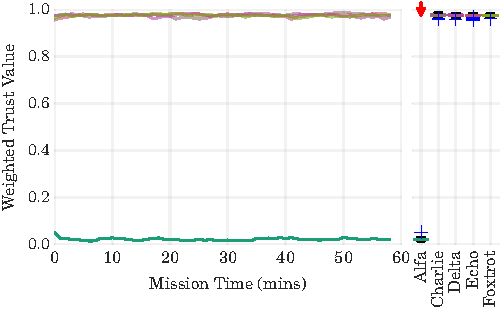
\includegraphics[width=\linewidth]{best_comms_run_time_MPC}
	  \caption{\gls{mpc} Comms Metric Trust }
	  \label{fig:comms_time_mpc}
	\end{subfigure}
	\begin{subfigure}[b]{0.5\textwidth}
		\centering
		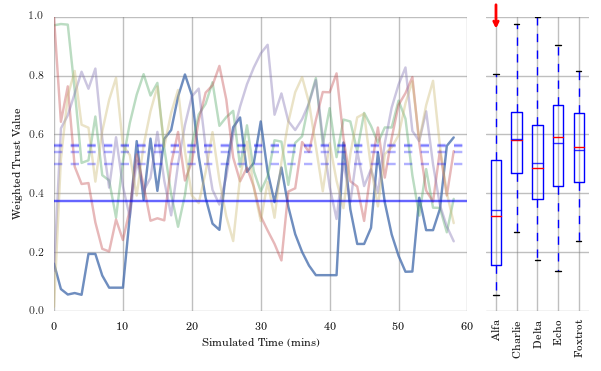
\includegraphics[width=\linewidth]{best_comms_run_time_STS}
		\caption{\gls{sts} Comms Metric Trust }
		\label{fig:comms_time_sts}
	\end{subfigure}
	
	\begin{subfigure}[b]{0.5\textwidth}
	  \centering
	  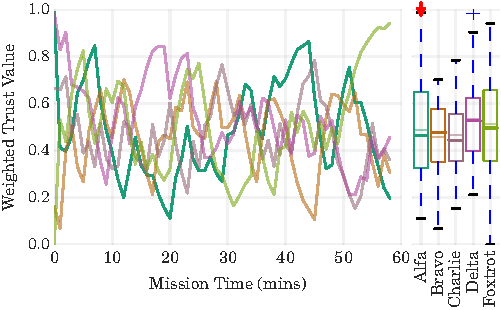
\includegraphics[width=\linewidth]{best_phys_run_time_MPC}
	  \caption{\gls{mpc} Physical Metric Trust }
	  \label{fig:phys_time_mpc}
	\end{subfigure}
	\begin{subfigure}[b]{0.5\textwidth}
		\centering
		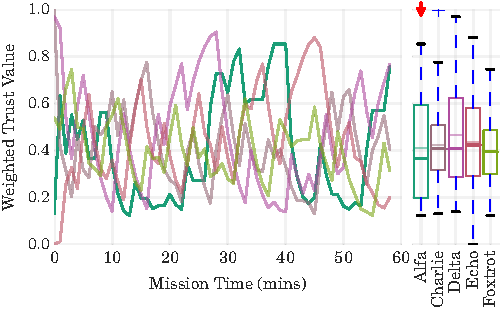
\includegraphics[width=\linewidth]{best_phys_run_time_STS}
		\caption{\gls{sts} Physical Metric Trust }
		\label{fig:phys_time_sts}
	\end{subfigure}
	
	\begin{subfigure}[b]{0.5\textwidth}
	  \centering
	  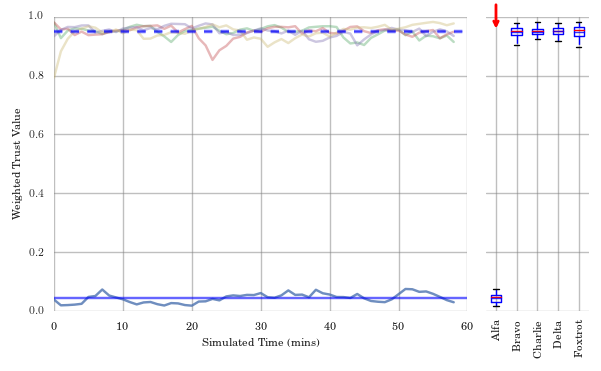
\includegraphics[width=\linewidth]{best_full_run_time_MPC}
	  \caption{\gls{mpc} Full Metric Trust }
	  \label{fig:full_time_mpc}
	\end{subfigure}
	\begin{subfigure}[b]{0.5\textwidth}
	  \centering
	  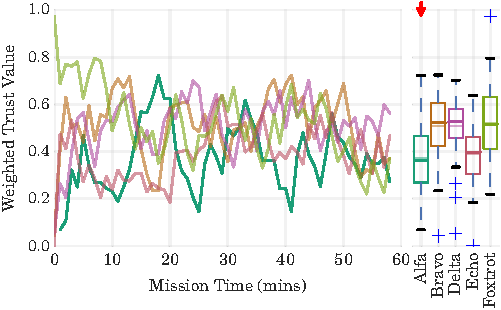
\includegraphics[width=\linewidth]{best_full_run_time_STS}
	  \caption{\gls{sts} Full Metric Trust }
	  \label{fig:full_time_sts}
	\end{subfigure}
	\caption{$T^{MTFM}$ assessments for \gls{mpc} and \gls{sts} ``Communications'' behaviours}
	\label{fig:trust_mpc_sts}
\end{figure}


\begin{figure}
	\begin{subfigure}[b]{0.5\textwidth}
		\centering
		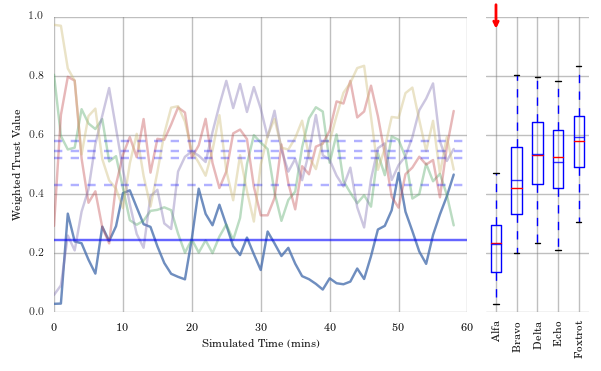
\includegraphics[width=\linewidth]{best_comms_run_time_Shadow}
		\caption{Shadow Comms Metric Trust}
		\label{fig:comms_time_shadow}
	\end{subfigure}
	\begin{subfigure}[b]{0.5\textwidth}
		\centering
		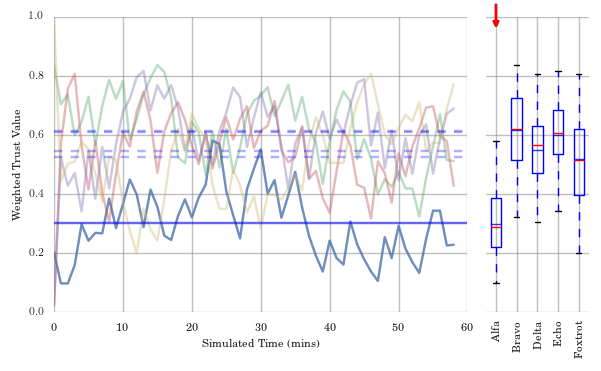
\includegraphics[width=\linewidth]{best_comms_run_time_SlowCoach}
		\caption{SlowCoach Comms Metric Trust}
		\label{fig:comms_time_slowcoach}
	\end{subfigure}
	
	\begin{subfigure}[b]{0.5\textwidth}
		\centering
		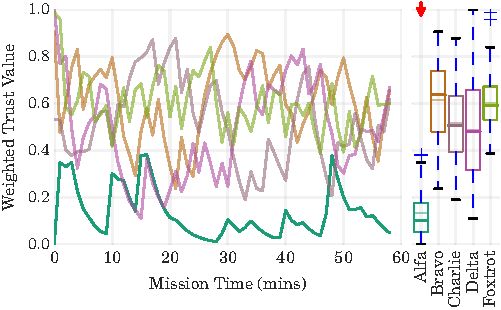
\includegraphics[width=\linewidth]{best_phys_run_time_Shadow}
		\caption{Shadow Physical Metric Trust }
		\label{fig:phys_time_shadow}
	\end{subfigure}
	\begin{subfigure}[b]{0.5\textwidth}
		\centering
		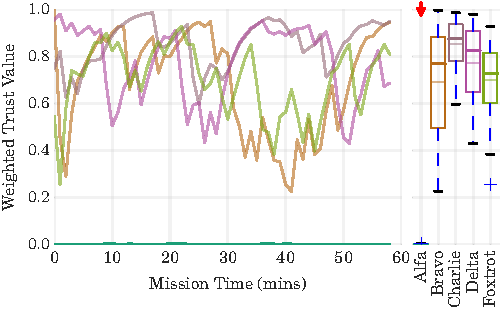
\includegraphics[width=\linewidth]{best_phys_run_time_SlowCoach}
		\caption{SlowCoach Physical Metric Trust}
		\label{fig:phys_time_slowcoach}
	\end{subfigure}
		
	\begin{subfigure}[b]{0.5\textwidth}
		\centering
		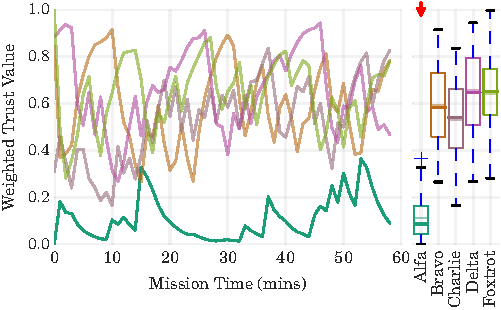
\includegraphics[width=\linewidth]{best_full_run_time_Shadow}
		\caption{Shadow Full Metric Trust }
		\label{fig:full_time_shadow}
	\end{subfigure}
	\begin{subfigure}[b]{0.5\textwidth}
		\centering
		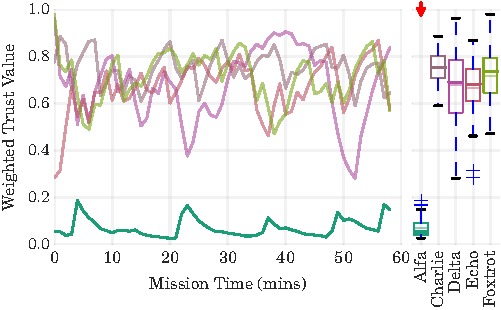
\includegraphics[width=\linewidth]{best_full_run_time_SlowCoach}
		\caption{SlowCoach Full Metric Trust}
		\label{fig:full_time_slowcoach}
	\end{subfigure}
	\caption{$T^{MTFM}$ assessments for Shadow and SlowCoach ``Physical'' behaviours}
	\label{fig:trust_shadow_slowcoach}
\end{figure}



	
% These tables are the output of test_Thesis_Diagrams.ThesisDiagrams#test0ValidationBestPlots
\begin{table}
	\centering
	\caption{$\Delta T$ across domains and ``proposed'' behaviours targeting known misbehaving node}
	%\begin{tabular}{|l|*{4}{c}|r|}
\toprule
\diagbox{Domain}{Behaviour} &  MPC &   STS &  Shadow &  SlowCoach &  Avg. \\
\midrule
Full       & 0.81 & -0.03 &    0.42 &       0.60 &  0.45 \\
Comms      & 0.85 &  0.04 &    0.19 &       0.26 &  0.34 \\
Phys       & 0.04 &  0.00 &    0.39 &       0.69 &  0.28 \\
Comms alt. & 0.85 &  0.03 &    0.38 &       0.45 &  0.43 \\
\hline
Phys alt.  & 0.48 &  0.03 &    0.42 &       0.63 &  0.39 \\
\bottomrule
\end{tabular}

	\begin{tabular}{|l|*{4}{c}|r|}
		\toprule
		\diagbox{Domain}{Behaviour} &  MPC &   STS &  Shadow &  SlowCoach &  Avg. \\
		\midrule
		Full       & 0.81 & -0.03 &    0.42 &       0.60 &  0.45 \\
		Comms      & 0.85 &  0.04 &    0.19 &       0.26 &  0.34 \\
		Phys       & 0.04 &  0.00 &    0.39 &       0.69 &  0.28 \\
		Comms alt. & 0.85 &  0.03 &    0.38 &       0.45 &  0.43 \\
		Phys alt.  & 0.48 &  0.03 &    0.42 &       0.63 &  0.39 \\
		\bottomrule
	\end{tabular}
	\label{tab:domain_deltas}
\end{table}

\begin{table}
	\centering
	\caption{$\Delta T^-$ False Positive assessments across domains and ``proposed'' behaviours across non-misbehaving nodes}
	%	\begin{tabular}{|l|*{4}{c}|r|}
\toprule
\diagbox{Domain}{Behaviour} &   MPC &   STS &  Shadow &  SlowCoach &  Avg. \\
\midrule
full      & -0.16 &  0.01 &   -0.08 &      -0.12 & -0.09 \\
comms     & -0.17 & -0.01 &   -0.04 &      -0.05 & -0.07 \\
phys      & -0.01 & -0.00 &   -0.08 &      -0.14 & -0.06 \\
comms\_alt & -0.17 & -0.01 &   -0.08 &      -0.09 & -0.09 \\
\hline
phys\_alt  & -0.10 & -0.01 &   -0.08 &      -0.13 & -0.08 \\
\bottomrule
\end{tabular}

	\begin{tabular}{|l|*{4}{c}|r|}
		\toprule
		\diagbox{Domain}{Behaviour} &   MPC &   STS &  Shadow &  SlowCoach &  Avg. \\
		\midrule
		Full       & -0.16 &  0.01 &   -0.08 &      -0.12 & -0.09 \\
		Comms      & -0.17 & -0.01 &   -0.04 &      -0.05 & -0.07 \\
		Phys       & -0.01 & -0.00 &   -0.08 &      -0.14 & -0.06 \\
		Comms alt. & -0.17 & -0.01 &   -0.08 &      -0.09 & -0.09 \\
		Phys alt.  & -0.10 & -0.01 &   -0.08 &      -0.13 & -0.08 \\
		\bottomrule
	\end{tabular}
	
	\label{tab:domain_deltas_minus}
\end{table}
%\todo{FIX CODE: These tables need changed from being ``delta T'' to ``Probability of detection by an idiotic classifier}

\begin{landscape}
  \begin{table}
    \centering
    \caption{Optimised metric vector weights per domain trained upon and behaviour targeted}
    \begin{tabular}{|l|l|*{9}{c|}}
\toprule
\multicolumn{2}{|c|}{\diagbox{Domain, Behaviour}{Metric}}     &  $Delay$ &  $P_{RX}$ &  $P_{TX}$ &    $S$ &    $G$ &  $PLR$ &  $INDD$ &  $INHD$ &  $Speed$ \\
\midrule
Full & MPC &   -0.033 &     0.154 &     0.495 &  0.034 & -0.035 &  0.062 &  -0.047 &  -0.039 &   -0.101 \\
     & STS &   -0.106 &     0.042 &     0.010 &  0.095 &  0.438 &  0.010 &  -0.194 &  -0.049 &   -0.055 \\
     & Shadow &    0.019 &     0.656 &     0.007 & -0.030 & -0.021 &  0.007 &  -0.081 &  -0.054 &   -0.125 \\
     & SlowCoach &    0.040 &     0.373 &     0.009 & -0.042 & -0.025 &  0.009 &  -0.087 &   0.099 &   -0.316 \\
\midrule
Comms & MPC &    0.045 &     0.068 &     0.665 &  0.029 & -0.043 &  0.150 &      &      &       \\
     & STS &    0.098 &     0.083 &     0.047 &  0.118 & -0.608 &  0.046 &      &      &       \\
     & Shadow &   -0.358 &     0.279 &     0.025 &  0.119 &  0.193 &  0.024 &      &      &       \\
     & SlowCoach &   -0.082 &     0.309 &     0.021 &  0.090 &  0.478 &  0.020 &      &      &       \\
\midrule
Phys & MPC &       &        &        &     &     &     &  -0.439 &  -0.383 &   -0.178 \\
     & STS &       &        &        &     &     &     &  -0.729 &  -0.164 &   -0.108 \\
     & Shadow &       &        &        &     &     &     &  -0.555 &  -0.142 &   -0.304 \\
     & SlowCoach &       &        &        &     &     &     &  -0.285 &  -0.118 &   -0.597 \\
\midrule
Comms alt. & MPC &       &        &     0.731 &  0.019 & -0.024 &  0.211 &  -0.014 &      &       \\
     & STS &       &        &     0.040 & -0.131 & -0.444 &  0.038 &  -0.348 &      &       \\
     & Shadow &       &        &     0.033 & -0.124 & -0.104 &  0.032 &  -0.707 &      &       \\
     & SlowCoach &       &        &     0.029 & -0.164 & -0.184 &  0.028 &  -0.595 &      &       \\
\midrule
Phys alt. & MPC &    0.043 &     0.389 &        &     &     &     &  -0.311 &  -0.075 &   -0.183 \\
     & STS &   -0.356 &     0.095 &        &     &     &     &  -0.235 &  -0.135 &   -0.179 \\
     & Shadow &    0.081 &     0.577 &        &     &     &     &  -0.097 &   0.070 &   -0.175 \\
     & SlowCoach &   -0.106 &     0.309 &        &     &     &     &  -0.067 &   0.099 &   -0.420 \\
\bottomrule
\end{tabular}

    \label{tab:optimised_weights}
  \end{table}
\end{landscape}

\section{Performance of Generalised Synthetic Domains}\label{sec:mdt_synthetic}
So far, the ability to generate and test the ``best'' metric weighting schemes across domains has been demonstrated, optimising for the highest levels of selectivity between fair and expected misbehaviours. 
However, these metric weighting schemes have been constructed into ``domains'' based on natural experience in the operating environment. 
Through observation of the metric significances shown in \autoref{fig:multi_feature_extraction}, potential alternative ``domains'' were generated through simple observation of the visual result.
In order to remove the human element, and investigate the wider impact and potential optimisation of this ``optimum subdomain'' subset idea, the idea whether these intrinsic  domains (Physical and Communications) can be improved upon by removing the assumption that ``Communications'' behaviours are best identified through the use of Communications metrics is tested.

To accomplish this, the discussed analysis from metric weight significance regression and generation to $\Delta{T}_{ix}$ and $\Delta{T}_{ix}^-$ validation is performed for all combinations of the $M=9$ explored metrics with three or more metrics ($k\ge3$). 

From this brute-force approach~\footnote{each ``run'' consisting of ${M\choose{k}}$ individual weight assessments, with the same multiplicity of 8 experimental runs per scenario per target node as before in previous runs}, a small investigation can be made in to both the performance of metric subsets, and the potential redundancies between metrics. 
For instance, one could expect that $P_{RX}$ would be almost always directly related to the expected positioning between nodes and therefore to \gls{indd}.
However, a counter hypothesis would be that this redundancy is present in the ``Fair'' case, but in misbehaving cases, the discrepancy between $P_{RX}$ and \gls{indd} could indicate or characterise a particular misbehaviour. 

\begin{figure}
	\begin{subfigure}[b]{0.5\textwidth}
		\centering
		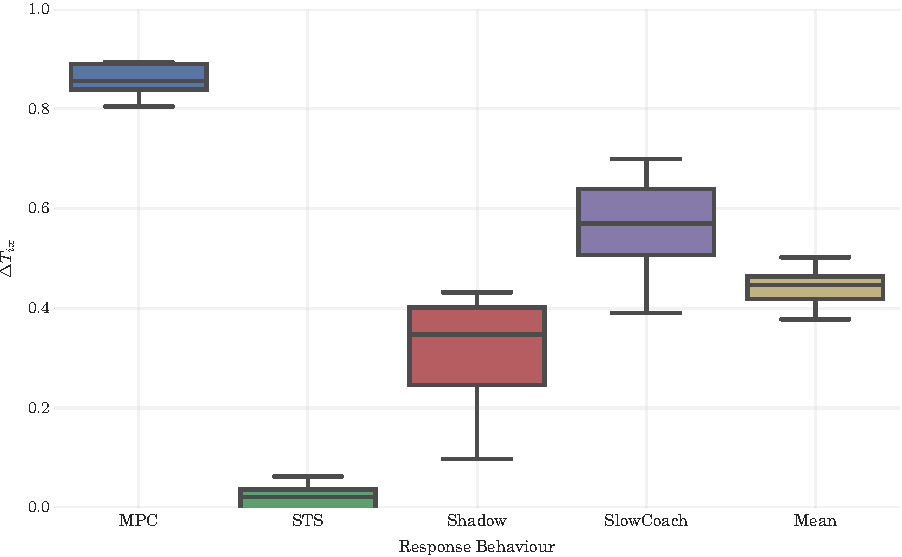
\includegraphics[width=\linewidth]{top_mpc_dt_box}
		\caption{MPC}
		\label{fig:top_mpc_dt_box}
	\end{subfigure}
	\begin{subfigure}[b]{0.5\textwidth}
		\centering
		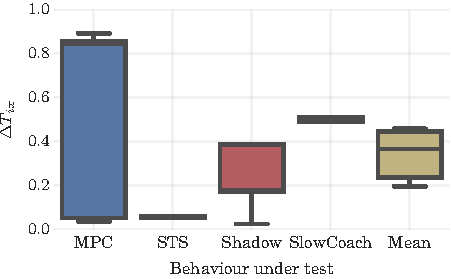
\includegraphics[width=\linewidth]{top_sts_dt_box}
		\caption{STS}
		\label{fig:top_sts_dt_box}
	\end{subfigure}\\
	
	\begin{subfigure}[b]{0.5\textwidth}
		\centering
		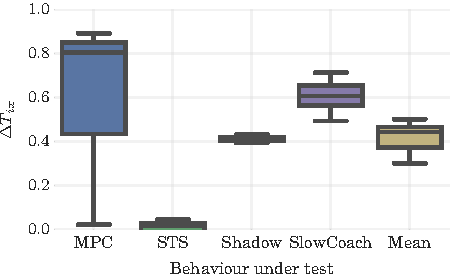
\includegraphics[width=\linewidth]{top_shadow_dt_box}
		\caption{Shadow}
		\label{fig:top_shadow_dt_box}
	\end{subfigure}
	\begin{subfigure}[b]{0.5\textwidth}
		\centering
		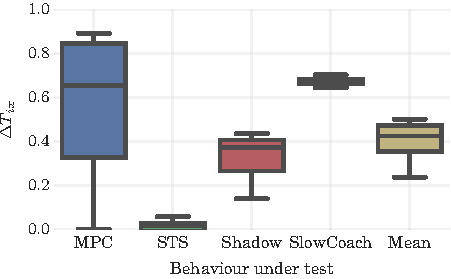
\includegraphics[width=\linewidth]{top_slowcoach_dt_box}
		\caption{SlowCoach}
		\label{fig:top_slowcoach_dt_box}
	\end{subfigure}
	
	\centering
	\begin{subfigure}[b]{0.5\textwidth}
		\centering
		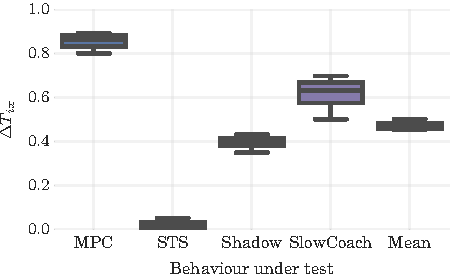
\includegraphics[width=\linewidth]{top_mean_dt_box}
		\caption{Mean of all responses}
		\label{fig:top_mean_dt_box}
	\end{subfigure}
	\caption{Variability in cross-behaviour performance of Top 10\% of synthetic domains based on individual misbehaviours and the overall mean response}\label{fig:top_dt_boxes}
\end{figure}

The True Positive ($\Delta T_{ix}$) is again used to indicate the overall performance of a particular synthetic domain (i.e. a synthetic domain created by the arbitrary selection of a given set of trust metrics for optimisation and assessment).
\autoref{fig:top_mean_dt_box} shows the distribution in $\Delta T_{ix}$ for each behaviour for the top 10\% of this simple mean.
As has been shown before, it's immediately clear that \gls{mpc} and SlowCoach are the more responsive behaviours to detect across the metric space, with Shadow being slightly more difficult and \gls{sts} remaining as challenging to detect as in earlier attempts.
This is disappointing, as it was hoped that \emph{some} combination of metrics in relative isolation would be capable of highlighting this behaviour in a more convincing manner, but it is clear that the Application level nature of the \gls{sts} attack is avoiding significant impacts across all the metrics currently applied.

Across the figures in \autoref{fig:top_dt_boxes}, when behaviours are targeted for this meta-optimisation, naive as it is, the variability in response performance in other, unoptimised, misbehaviours is greatly increased, indicating that, at least in the case of attempting to \emph{identify} misbehaviour, that this is a case of over-optimisation, and that in the majority of cases, optimising for the mean response (\autoref{fig:top_mean_dt_box}) will be sufficient to get a strong and consistent performance across misbehaviours.

This is shown explicitly in \autoref{fig:focus_ratio}, where the selective performance ratio between a targeted subset optimisation and the ``mean'' subset optimisation demonstrates that in all cases but \gls{sts}, targeting specific behaviours for this domain synthesis does not meaningfully improve the true-positive behaviour of trust assessment, and in general decreases the detection accuracy.
The abstractions for the generation of \autoref{fig:focus_ratio} are shown in \autoref{tab:focus_ratio}.

Looking at the performance of these targeted synthetic domains with respect to the metrics used, \autoref{fig:top_targeted_dt_heatmap} shows the metric selection correlations across metrics and behaviours.
From this it is observed that while there is a relatively consistent relationship between ``Physical'' metrics (\gls{indd}, \gls{inhd} and Speed) and ``Physical'' misbehaviours (SlowCoach and Shadow), this is far from consistent across the domain space. 

Looking back at the performance of the previously used Native and Alternative Domains, \autoref{tab:domain_deltas} can be extended to include results from the ``Best'' synthetic domains for each misbehaviour, shown in \autoref{tab:augmented_domain_deltas}.
As stated, it is not surprising that these Behaviour-optimised synthetic domains perform better at maximising $\Delta T_{ix}$ in their targeted behaviours, with an incurred reduction in the average response to other misbehaviours. 

In terms of a comparison between the previously generated ``Alternate'' domains, which were made by visual inspection of the returned relevance from \autoref{fig:multi_feature_extraction}, the ``SlowCoach'' synthetic domain uses almost all the same domains as the ``Phys Alt.'' domain, such that the synthetic domain leaves the Delay metric out, and in all cases except for \gls{sts}, outperforms the Alternate domain.


\begin{table}
	\centering
	\caption{Top 5 performing synthetic domains, targeting MPC, and including their performance in detecting other misbehaviours}
	\centerline{\begin{tabular}{|*{5}{c|}|*{9}{c|}}
\toprule
\multicolumn{5}{|c||}{Behaviour $\Delta T_{ix}$} & \multicolumn{9}{c|}{Metrics in Synthetic Domain}\\
               MPC &   STS & Shadow & SlowCoach & Mean &                     $Delay$ & $P_{RX}$ & $P_{TX}$ &  $S$ &  $G$ & $PLR$ & $INDD$ & $INHD$ & $Speed$ \\
\midrule
              0.89 &  0.01 &   0.35 &      0.54 & 0.45 &                        1.00 &     1.00 &     1.00 & 0.00 & 0.00 &  0.00 &   0.00 &   1.00 &    0.00 \\
              0.89 & -0.03 &   0.17 &      0.64 & 0.42 &                        1.00 &     0.00 &     1.00 & 0.00 & 1.00 &  0.00 &   0.00 &   1.00 &    1.00 \\
              0.89 &  0.05 &   0.12 &      0.46 & 0.38 &                        1.00 &     0.00 &     1.00 & 1.00 & 0.00 &  0.00 &   0.00 &   1.00 &    0.00 \\
              0.89 &  0.04 &   0.35 &      0.55 & 0.46 &                        1.00 &     1.00 &     1.00 & 1.00 & 0.00 &  0.00 &   0.00 &   1.00 &    0.00 \\
              0.89 & -0.03 &   0.27 &      0.49 & 0.41 &                        0.00 &     0.00 &     1.00 & 1.00 & 0.00 &  0.00 &   1.00 &   1.00 &    0.00 \\
\bottomrule
\end{tabular}
}
	\label{tab:top_mpc_dt}
\end{table}
\begin{table}
	\centering
	\caption{As in \autoref{tab:top_mpc_dt}, but targeting STS}
	\centerline{\begin{tabular}{|*{5}{c|}|*{9}{c|}}
\toprule
\multicolumn{5}{|c||}{Behaviour $\Delta T_{ix}$} & \multicolumn{9}{c|}{Metrics in Synthetic Domain}\\
               MPC &  STS & Shadow & SlowCoach & Mean &                     $Delay$ & $P_{RX}$ & $P_{TX}$ &  $S$ &  $G$ & $PLR$ & $INDD$ & $INHD$ & $Speed$ \\
\midrule
              0.86 & 0.06 &   0.37 &      0.49 & 0.45 &                         \OK &          &      \OK &  \OK &      &   \OK &    \OK &        &         \\
              0.84 & 0.06 &   0.39 &      0.51 & 0.45 &                         \OK &          &      \OK &      &      &   \OK &    \OK &        &         \\
              0.83 & 0.06 &   0.03 &      0.02 & 0.23 &                         \OK &          &      \OK &  \OK &      &   \OK &        &        &         \\
              0.04 & 0.06 &   0.18 &      0.68 & 0.24 &                         \OK &          &          &      &  \OK &   \OK &        &        &     \OK \\
              0.05 & 0.06 &   0.17 &      0.51 & 0.20 &                         \OK &          &          &      &      &   \OK &        &    \OK &     \OK \\
\bottomrule
\end{tabular}
}
	\label{tab:top_sts_dt}
\end{table}
\begin{table}
	\centering
	\caption{As in \autoref{tab:top_mpc_dt}, but targeting Shadow}
	\centerline{\begin{tabular}{|*{5}{c|}|*{9}{c|}}
\toprule
\multicolumn{5}{|c||}{Behaviour $\Delta T_{ix}$} & \multicolumn{9}{c|}{Metrics in Synthetic Domain}\\
               MPC &   STS & Shadow & SlowCoach & Mean &                     $Delay$ & $P_{RX}$ & $P_{TX}$ & $S$ & $G$ & $PLR$ & $INDD$ & $INHD$ & $Speed$ \\
\midrule
              0.49 & -0.00 &   0.44 &      0.66 & 0.40 &                             &      \OK &          &     &     &       &    \OK &    \OK &     \OK \\
              0.81 & -0.03 &   0.43 &      0.68 & 0.47 &                             &      \OK &      \OK &     &     &   \OK &    \OK &        &     \OK \\
              0.81 &  0.02 &   0.43 &      0.66 & 0.48 &                         \OK &      \OK &      \OK &     &     &   \OK &    \OK &        &     \OK \\
              0.78 & -0.02 &   0.43 &      0.62 & 0.45 &                             &      \OK &      \OK &     &     &   \OK &    \OK &    \OK &     \OK \\
              0.40 & -0.01 &   0.43 &      0.63 & 0.36 &                             &      \OK &          &     &     &   \OK &    \OK &    \OK &     \OK \\
\bottomrule
\end{tabular}
}
	\label{tab:top_shadow_dt}
\end{table}
\begin{table}
	\centering
	\caption{As in \autoref{tab:top_mpc_dt}, but targeting SlowCoach}
	\centerline{\begin{tabular}{|*{5}{c|}|*{9}{c|}}
\toprule
\multicolumn{5}{|c||}{Behaviour $\Delta T_{ix}$} & \multicolumn{9}{c|}{Metrics in Synthetic Domain}\\
               MPC &   STS & Shadow & SlowCoach & Mean &                     $Delay$ & $P_{RX}$ & $P_{TX}$ &  $S$ &  $G$ & $PLR$ & $INDD$ & $INHD$ & $Speed$ \\
\midrule
              0.47 &  0.00 &   0.37 &      0.72 & 0.39 &                         \OK &      \OK &          &  \OK &      &       &        &        &     \OK \\
              0.67 & -0.03 &   0.39 &      0.72 & 0.44 &                         \OK &      \OK &          &      &  \OK &       &        &        &     \OK \\
              0.52 &  0.02 &   0.42 &      0.71 & 0.42 &                             &      \OK &          &      &  \OK &       &    \OK &        &     \OK \\
              0.37 &  0.03 &   0.40 &      0.71 & 0.38 &                         \OK &      \OK &          &      &      &       &    \OK &        &     \OK \\
              0.33 & -0.02 &   0.40 &      0.71 & 0.36 &                             &      \OK &          &  \OK &      &       &    \OK &        &     \OK \\
\bottomrule
\end{tabular}
}
	\label{tab:top_slowcoach_dt}
\end{table}
\begin{table}
	\centering
	\caption{As in \autoref{tab:top_mpc_dt}, but targeting the mean response across misbehaviours}
	\centerline{\begin{tabular}{|*{5}{c|}|*{9}{c|}}
\toprule
\multicolumn{5}{|c||}{Behaviour $\Delta T_{ix}$} & \multicolumn{9}{c|}{Metrics in Synthetic Domain}\\
               MPC &  STS & Shadow & SlowCoach & Mean &                     $Delay$ & $P_{RX}$ & $P_{TX}$ &  $S$ &  $G$ & $PLR$ & $INDD$ & $INHD$ & $Speed$ \\
\midrule
              0.88 & 0.03 &   0.42 &      0.69 & 0.50 &                             &      \OK &      \OK &      &  \OK &       &    \OK &        &     \OK \\
              0.87 & 0.03 &   0.42 &      0.68 & 0.50 &                         \OK &      \OK &      \OK &      &  \OK &       &    \OK &        &     \OK \\
              0.89 & 0.04 &   0.37 &      0.69 & 0.50 &                             &      \OK &      \OK &      &  \OK &       &        &        &     \OK \\
              0.87 & 0.02 &   0.42 &      0.67 & 0.50 &                         \OK &      \OK &      \OK &      &      &       &    \OK &        &     \OK \\
              0.88 & 0.04 &   0.38 &      0.68 & 0.49 &                             &      \OK &      \OK &  \OK &  \OK &       &        &        &     \OK \\
\bottomrule
\end{tabular}
}
	\label{tab:top_mean_dt}
\end{table}

\begin{table}
	\centering
	\caption{Averaged summary of top 10\% for each targeted behaviour, with the average ratio of occurrence of each metrics for the summarised synthetic domains}
	
	%\centerline{\begin{tabular}{|*{5}{c|}|*{9}{c|}}
\toprule
\multicolumn{5}{|c||}{Behaviour $\Delta T_{ix}$} & \multicolumn{9}{c|}{Metrics in Synthetic Domain}\\
               MPC &  STS & Shadow & SlowCoach & Mean &                     $Delay$ & $P_{RX}$ & $P_{TX}$ &  $S$ &  $G$ & $PLR$ & $INDD$ & $INHD$ & $Speed$ \\
                   &      &        &           &      &                             &          &          &      &      &       &        &        &         \\
\midrule
              0.89 & 0.02 &   0.25 &      0.53 & 0.42 &                        0.65 &     0.40 &     1.00 & 0.50 & 0.40 &  0.00 &   0.20 &   0.70 &    0.45 \\
              0.58 & 0.05 &   0.25 &      0.43 & 0.33 &                        0.80 &     0.40 &     0.55 & 0.70 & 0.30 &  0.65 &   0.30 &   0.35 &    0.35 \\
              0.70 & 0.00 &   0.43 &      0.63 & 0.44 &                        0.50 &     1.00 &     0.65 & 0.05 & 0.45 &  0.75 &   1.00 &   0.70 &    0.95 \\
              0.52 & 0.00 &   0.38 &      0.70 & 0.40 &                        0.50 &     0.80 &     0.25 & 0.35 & 0.65 &  0.15 &   0.65 &   0.05 &    1.00 \\
              0.87 & 0.02 &   0.40 &      0.67 & 0.49 &                        0.55 &     1.00 &     1.00 & 0.35 & 0.70 &  0.20 &   0.60 &   0.20 &    1.00 \\
\bottomrule
\end{tabular}
}
	\centerline{\begin{tabular}{|p{2cm}||*{5}{c|}|*{9}{c|}}
		\toprule
		\multirow{3}{*}{\parbox{2cm}{Targeted Behaviour}}&\multicolumn{5}{c||}{Behaviour $\Delta T_{ix}$} & \multicolumn{9}{c|}{Metrics in Synthetic Domain}\\
			 &                \rot{MPC} &  \rot{STS} & \rot{Shadow} & \rot{SlowCoach} & \rot{Mean} &                     \rot{$Delay$} & \rot{$P_{RX}$} & \rot{$P_{TX}$} &  \rot{$S$} &  \rot{$G$} & \rot{$PLR$} & \rot{$INDD$} & \rot{$INHD$} & \rot{$Speed$} \\
		\midrule
		MPC                &               0.89 & 0.02 &   0.25 &      0.53 & 0.42 &                        0.65 &     0.40 &     1.00 & 0.50 & 0.40 &  0.00 &   0.20 &   0.70 &    0.45 \\
		STS                &               0.58 & 0.05 &   0.25 &      0.43 & 0.33 &                        0.80 &     0.40 &     0.55 & 0.70 & 0.30 &  0.65 &   0.30 &   0.35 &    0.35 \\
		Shadow             &               0.70 & 0.00 &   0.43 &      0.63 & 0.44 &                        0.50 &     1.00 &     0.65 & 0.05 & 0.45 &  0.75 &   1.00 &   0.70 &    0.95 \\
		SlowCoach          &               0.52 & 0.00 &   0.38 &      0.70 & 0.40 &                        0.50 &     0.80 &     0.25 & 0.35 & 0.65 &  0.15 &   0.65 &   0.05 &    1.00 \\
		Mean               &               0.87 & 0.02 &   0.40 &      0.67 & 0.49 &                        0.55 &     1.00 &     1.00 & 0.35 & 0.70 &  0.20 &   0.60 &   0.20 &    1.00 \\
		\bottomrule
	\end{tabular}}

	\label{tab:focus_ratio}
\end{table}

\begin{figure}
	\centering
	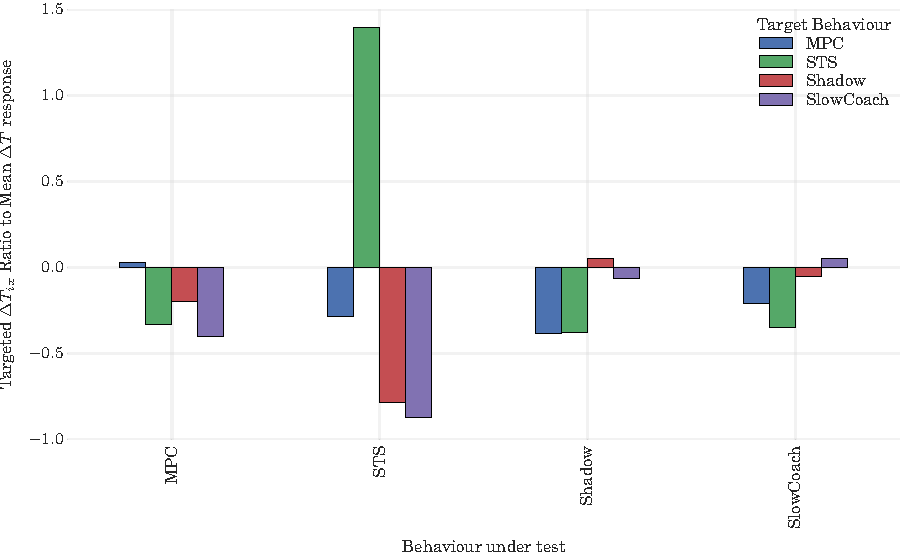
\includegraphics[width=0.8\linewidth]{focus_ratio}
	\caption{Ratio of relative per-behaviour synthetic domain targeting to Mean targeting}
	\label{fig:focus_ratio}
\end{figure}

\begin{figure}
	\centering
	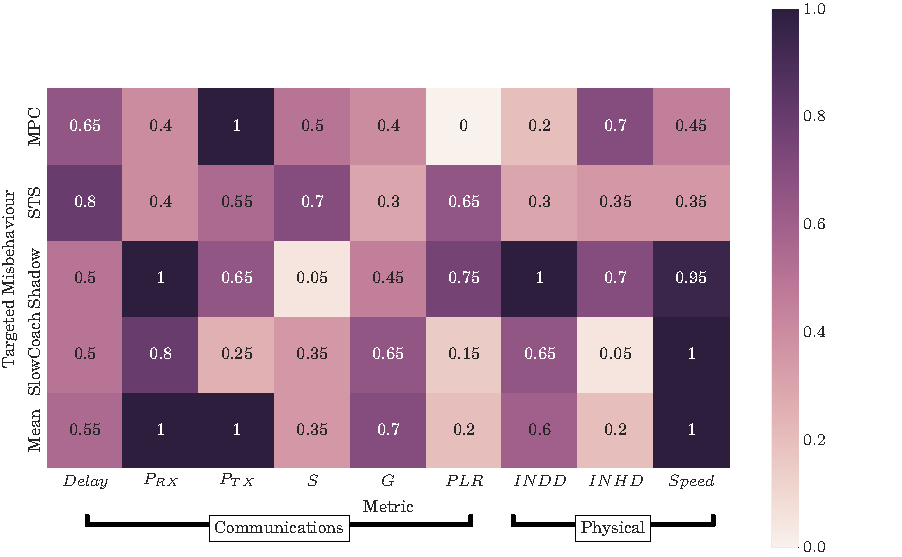
\includegraphics[width=0.8\linewidth]{top_targeted_dt_heatmap}
	\caption{Correlations between highest performing synthetic domain metrics with respect to Targeted misbehaviours}
	\label{fig:top_targeted_dt_heatmap}
\end{figure}

\begin{table}
	\centering
	\caption{$\Delta T_{ix}$ behaviour detection performance across basic, alternate, and targeted-synthetic domains, showing the respective constituent metrics}
	{\renewcommand{\arraystretch}{1.1} 
	\begin{tabular}{|c p{2cm}||*{5}{c|}|*{9}{c|}}
		\toprule
		\multicolumn{2}{|c||}{\multirow{3}{*}{\parbox{2cm}{Domain}}}&\multicolumn{5}{c||}{Behaviour $\Delta T_{ix}$} & \multicolumn{9}{c|}{Metrics in Domain}\\
		&&                \rot{MPC} &  \rot{STS} & \rot{Shadow} & \rot{SlowCoach} & \rot{Mean} &                     \rot{$Delay$} & \rot{$P_{RX}$} & \rot{$P_{TX}$} &  \rot{$S$} &  \rot{$G$} & \rot{$PLR$} & \rot{$INDD$} & \rot{$INHD$} & \rot{$Speed$} \\
		\midrule
		\multirow{3}{*}{\rot{Basic}} & Full       & 0.81 & -0.03 &    0.42 &       0.60 &  0.45 &\OK&\OK&\OK&\OK&\OK&\OK&\OK&\OK&\OK\\
		& Comms      & 0.85 &  0.04 &    0.19 &       0.26 &  0.34 &\OK&\OK&\OK&\OK&\OK&\OK&&&\\
		& Phys       & 0.04 &  0.00 &    0.39 &       0.69 &  0.28 &&&&&&&\OK&\OK&\OK\\\hline
		\multirow{4}{*}{\rot{Alternate}}&&&&&&&&&&&&&&&\\[-0.8em]
		& Comms alt. & 0.85 &  0.03 &    0.38 &       0.45 &  0.43 &&&&\OK&\OK&\OK&\OK&&\\[0.2em]
		& Phys alt.  & 0.48 &  0.03 &    0.42 &       0.63 &  0.39 &\OK&\OK&&&&&\OK&\OK&\OK\\
		&&&&&&&&&&&&&&&\\[-0.5em]\hline
        \multirow{5}{*}{\rot{Synthetic}}&&&&&&&&&\\[-1em]
        & MPC        & 0.89 &  0.01 &   0.35 &      0.54 & 0.45 &                         \OK &      \OK &      \OK &      &      &       &        &    \OK &         \\
		& STS        & 0.86 & 0.06 &   0.37 &      0.49 & 0.45 &                         \OK &          &      \OK &  \OK &      &   \OK &    \OK &        &         \\
		& Shadow     & 0.49 & -0.00 &   0.44 &      0.66 & 0.40 &                             &      \OK &          &     &     &       &    \OK &    \OK &     \OK \\
		& SlowCoach  & 0.47 &  0.00 &   0.37 &      0.72 & 0.39 &                         \OK &      \OK &          &  \OK &      &       &        &        &     \OK \\
		& Mean       & 0.88 & 0.03 &   0.42 &      0.69 & 0.50 &                             &      \OK &      \OK &      &  \OK &       &    \OK &        &     \OK \\
		\bottomrule
	\end{tabular}}
	\label{tab:augmented_domain_deltas}
\end{table}

\section{Selectivity Performance of Optimised Domains}\label{sec:selectivity-performance-of-optimised-domains}

Having arrived at a set of Basic, Alternate, and now Synthetic domains, optimised for maximising the induced ``drop'' in trust, (i.e. maximising $\Delta T_{ix}$), an estimate of the actual performance of these assessments must be made.
This is accomplished using an extension of the Dixon classifier used in \autoref{ch:physical_trust}, such that rather than detecting outliers based on a physical metric, outliers are detected based on the differential trust value given by a given optimised weight.

This is initially tested in what can be considered the ``best case''; using the previously optimised domains above to weight a collection of over 5000 execution runs in each of the basic, alternate and synthetic domains, and using this multi-domain trust vector in Dixons' Q-Test. (Again, $Q^{95}$)

The results from this detection test are shown in \autoref{tab:synth_detect} and \autoref{tab:synth_detect}.
Comparing the synthetic domain results to the existing alternate and basic domains, in all cases except for SlowCoach, the targeted domain performs marginally better than any other domain, but the margin in this is very slim.

\gls{sts} continues to evade direct detection despite having promising metric and domain significances; across all metric weightings and domains applied, the 7\% detection rate arrived at with its synthetic domain (matching it's false positive rate) may be the best that can be expected from this methodology.

In the case where there is no misbehaviour, the targeted synthetic domain sets demonstrate a marginally smaller True Negative performance compared to the basic and alternate domains, with the exception of the Mean synthetic case, which is operationally equivalent in performance to the ``Full'' basic domain in terms of detecting the ``absence'' of misbehaviour. 
Considering that the Mean synthetic domain has just over half the number of engaged metrics of the Full domain (\autoref{tab:augmented_domain_deltas}), this would indicate that the Mean synthetic domain is a prime candidate for a ``general misbehaver detection'' domain with lower computational complexity than either re-running a full metric optimisation as per \autoref{ch:comms_trust} at runtime, or applying a suite of alternate or synthetic domains to perform an ensemble detection\footnote{It is interesting to note that this ``Mean'' synthetic domain does not contain \gls{plr}, which is the primary metric for most standard \gls{manet} \glspl{tmf}}.

\begin{table}
	\centering
	\caption{Accuracy of Correct identification of misbehaver using Domain-Trained weight vectors with a Dixons Q based limit-classifier}
	\label{tab:synth_detect}
	\begin{tabular}{|l p{2cm}||r|r|r|r|r|r|r|r|}
		\toprule
		\multicolumn{2}{|c||}{\multirow{3}{*}{\parbox{2cm}{Domain}}} &    \multicolumn{4}{c|}{\parbox{4cm}{\centering True Positive Identification of Misbehaver\vspace{.5\baselineskip}}} &    \multicolumn{4}{c|}{\parbox{4cm}{\centering False Positive Identification of Misbehaver\vspace{.5\baselineskip}}}    \\[0.3em]
		 &&   \rot{MPC} &  \rot{STS} & \rot{Shadow} & \rot{SlowCoach} &   \rot{MPC} &  \rot{STS} & \rot{Shadow} & \rot{SlowCoach} \\
		\midrule
		\multirow{4}{*}{\rot{Basic}}&&&&&&&&&\\[-1em]
		& Full          &  1.00 &  0.03 &   0.63 &      0.98 &  0.00 &  0.07 &   0.00 &       0.0 \\
		& Comms         &  1.00 &  0.05 &   0.18 &      0.39 &  0.00 &  0.03 &   0.04 &       0.0 \\
		& Phys          &  0.03 &  0.02 &   0.40 &      0.85 &  0.12 &  0.09 &   0.00 &       0.0 \\\hline
		\multirow{4}{*}{\rot{Alternate}}&&&&&&&&&\\[-0.8em]
		& Comms alt.    &  1.00 &  0.03 &   0.22 &      0.43 &  0.00 &  0.15 &   0.02 &       0.0 \\[0.2em]
		& Phys alt.     &  0.54 &  0.04 &   0.62 &      0.97 &  0.00 &  0.06 &   0.00 &       0.0 \\
		&&&&&&&&&\\[-0.5em]\hline
		\multirow{5}{*}{\rot{Synthetic}}&&&&&&&&&\\[-1em]
		& MPC           &  1.00 &  0.04 &   0.62 &      0.80 &  0.00 &  0.04 &   0.00 &       0.0 \\
		& STS           &  1.00 &  0.07 &   0.24 &      0.45 &  0.00 &  0.07 &   0.00 &       0.0 \\
		& Shadow        &  0.57 &  0.02 &   0.64 &      0.95 &  0.00 &  0.07 &   0.00 &       0.0 \\
		& SlowCoach     &  0.70 &  0.04 &   0.71 &      0.88 &  0.00 &  0.06 &   0.00 &       0.0 \\
		& Mean          &  1.00 &  0.02 &   0.70 &      0.93 &  0.00 &  0.12 &   0.00 &       0.0 \\
		\bottomrule
	\end{tabular}

\end{table}

\begin{table}
	\centering
	\caption{Negative-Accuracy of Correct identification of misbehaver using Domain-Trained weight vectors with a Dixons Q based limit-classifier}
	\label{tab:synth_detect_false}
	\begin{tabular}{|l p{2cm}||r|r|r|r|r|r|r|r|}
		\toprule
		\multicolumn{2}{|c||}{\multirow{3}{*}{\parbox{2cm}{Domain}}} &    \multicolumn{4}{c|}{\parbox{4cm}{\centering True Negative Identification of Misbehaver\vspace{.5\baselineskip}}} &    \multicolumn{4}{c|}{\parbox{4cm}{\centering False Negative Identification of Misbehaver\vspace{.5\baselineskip}}}    \\[0.3em]
		&&   \rot{MPC} &  \rot{STS} & \rot{Shadow} & \rot{SlowCoach} &   \rot{MPC} &  \rot{STS} & \rot{Shadow} & \rot{SlowCoach} \\
		\midrule
		\multirow{4}{*}{\rot{Basic}}&&&&&&&&&\\[-1em]
		& Full          &  0.90 &  0.86 &   0.92 &      0.91 &  0.13 &  0.15 &   0.11 &      0.12 \\
		& Comms         &  0.88 &  0.96 &   0.94 &      0.94 &  0.12 &  0.06 &   0.10 &      0.07 \\
		& Phys          &  0.90 &  0.93 &   0.90 &      0.87 &  0.12 &  0.07 &   0.10 &      0.18 \\\hline
		\multirow{4}{*}{\rot{Alternate}}&&&&&&&&&\\[-0.5em]
		& Comms alt.    &  0.92 &  0.95 &   0.88 &      0.89 &  0.10 &  0.08 &   0.14 &      0.12 \\[0.2em]
		& Phys alt.     &  0.90 &  0.89 &   0.95 &      0.92 &  0.13 &  0.14 &   0.06 &      0.11 \\
		&&&&&&&&&\\[-0.5em]\hline
		\multirow{5}{*}{\rot{Synthetic}}&&&&&&&&&\\[-1em]
		& MPC           &  0.86 &  0.92 &   0.90 &      0.96 &  0.19 &  0.11 &   0.13 &      0.06 \\
		& STS           &  0.93 &  0.95 &   0.87 &      0.86 &  0.09 &  0.10 &   0.15 &      0.16 \\
		& Shadow        &  0.90 &  0.90 &   0.91 &      0.93 &  0.14 &  0.11 &   0.13 &      0.10 \\
		& SlowCoach     &  0.92 &  0.89 &   0.92 &      0.91 &  0.11 &  0.15 &   0.13 &      0.13 \\
		& Mean          &  0.90 &  0.93 &   0.92 &      0.91 &  0.13 &  0.09 &   0.12 &      0.10 \\
		\bottomrule
		\bottomrule
	\end{tabular}

\end{table}

\begin{figure}
	\centering
	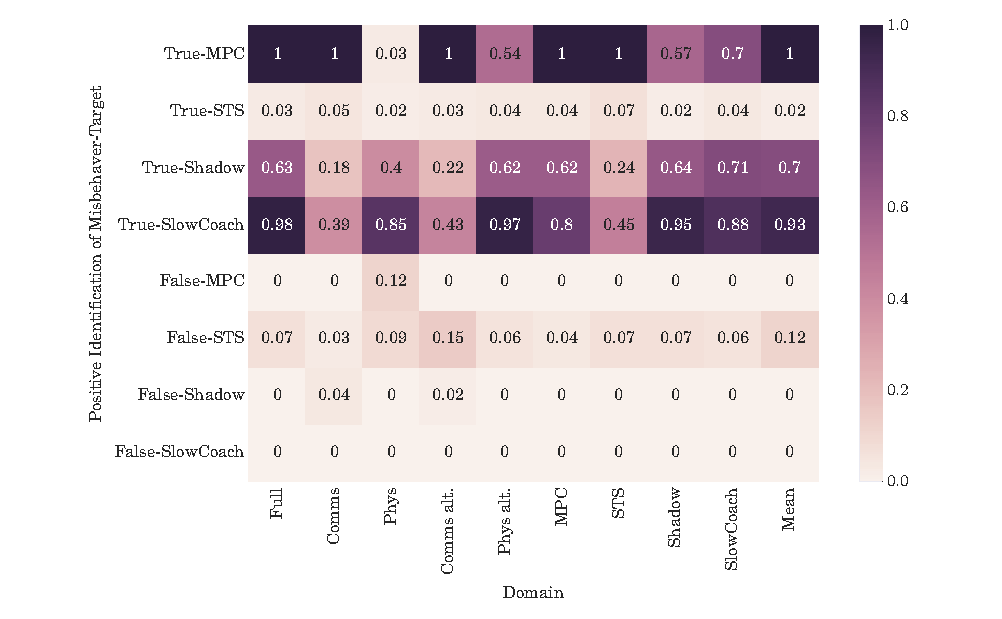
\includegraphics[width=\linewidth]{positive_heat}
	\caption{Accuracy of Correct identification of misbehaver using Domain-Trained weight vectors with a Dixons Q based limit-classifier}
	\label{fig:positive_heat}
\end{figure}

\begin{figure}
	\centering
	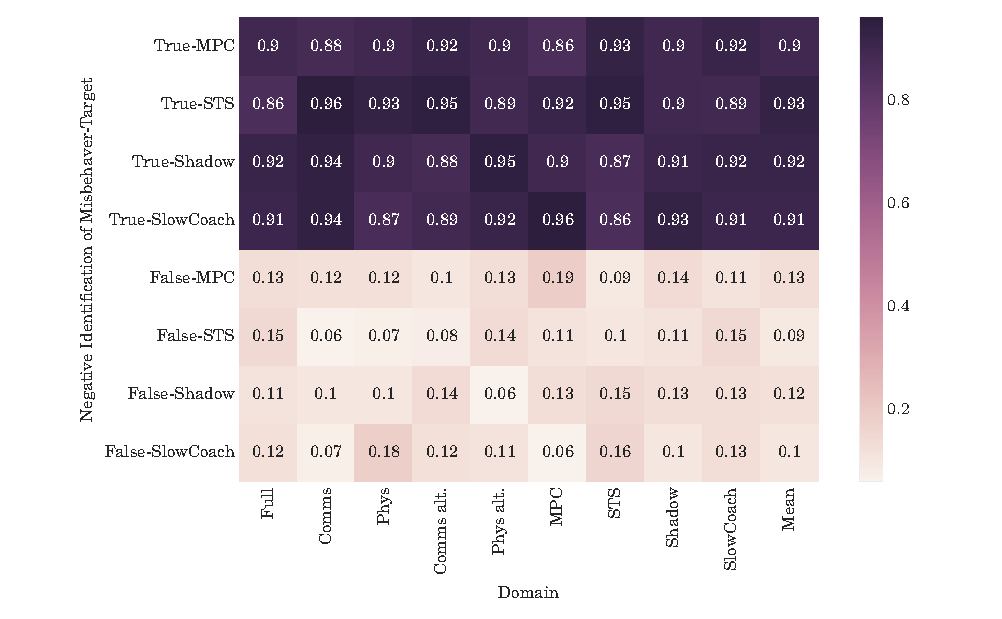
\includegraphics[width=\linewidth]{negative_heat}
	\caption{Negative-Accuracy of Correct identification of misbehaver using Domain-Trained weight vectors with a Dixons Q based limit-classifier}
	\label{fig:negative_heat}
\end{figure}


\section{Conclusion}

Key Outcomes: 
\begin{itemize}
	\item Demonstrated that (seemingly) domain-specific behaviours have detectable impacts across other domains (\autoref{sec:mdt_defined})
	\item \autoref{q:joint} - Demonstrated that combining communications and physical domains yields a functioning cross-domain \gls{tmf} (\autoref{sec:mdt_alternate})
	\item Demonstrated a generic method for generating optimised synthetic domains targeting particular behaviour to reduce computation requirements (\autoref{sec:mdt_synthetic})
	\item Demonstrated that per-misbehaviour synthetic domains out-perform all other domains in overall impact on resultant trust assessments (\autoref{tab:augmented_domain_deltas})
	\item Identified that the application-level \gls{sts} is particularly difficult to blindly classify despite high levels of metric significance (\autoref{sec:selectivity-performance-of-optimised-domains})
	\item \autoref{q:perf} - Demonstrated that in most cases, generalised synthetic domains outperform both Basic domains and human-judged Alternate domain groupings in misbehaviour detection and classification (\autoref{tab:synth_detect})
\end{itemize}

In this chapter we demonstrate that in harsh environments, multi-domain trust assessment can perform better on average than single-domain counterparts, both in terms of robustness and sensitivity, but also covering a wider region of the potential behaviour space, 

The extension of the methodologies of multi-vector trust into the marine space are already demonstrated, however including information from physical observations of actors in a network enables the detection and identification of a much wider range of behaviours.
We also demonstrate a method for assessing trust metrics in harsh environments in terms of their relative significance, and a method for establishing classification signatures for misbehaviours.
Finally, the synthetic generation of abstract metric domains is explored, where it is found that in most cases, optimising for generalised performance provides the strongest deviations in observed Trust when targeted specifically, further supporting the use of a mixed-domain approach for Trust across domains for identification of misbehaviours (\autoref{q:joint}, \autoref{q:perf}).

It is to be noted that this presented method is significantly more computationally intensive than the relatively simple Hermes / \gls{otmf} algorithms communications only algorithms, and is exponential in complexity as metrics and/or domains are added. The repeated metric re-weighting required for real time behaviour detection is therefore an area that requires optimization. More work needs to be done to characterise how worthwhile this approach is compared to a separate synthesis approach where by \gls{mtfm}-style trust is generated and assessed on a per-domain basis and subsequently fused.

Every effort has been made to avoid over-training the dataset, using cross validating sampling for regression and "best weight" generation, however more meta-analysis is required to further demonstrate the optimality of this process.

For greater fidelity and more optimal results, a wider range of weights can be used in the initial regression step; however this is computationally expensive given that weighting is applied to each perspective (i.e.\ observer/target node pair) for each trust assessment time step, presenting 15 perspectives at each time interval in the 6 node case.

For discrete detection of the presence of misbehaviours and identification of a misbehaver, it is shown that optimising for the $\Delta T_{ix}$ mean response across misbehaviours provides a domain with almost identical selectivity, which uses metrics from across both communications and physical domains to provide a general ``canary'' trust assessment, and with further exploration in to scenario and environmental applicability, could prove to be a viable ``first port of call'' synthetic domain.



%%%%%%%%%%%%%%%%%%%%%%%%%%%%%%%%%%%%%%%%%%%%%%%%%%%%%%%%%%%%%%%%%%%%%%%%%%%%%%%
